\lab{Polynomial Interpolation Using Chebyshev Polynomials}{Polynomial Interpolation Using Chebyshev Polynomials}
\label{lab:cheb_interp}

\objective{Explore basic uses of polynomial interpolation using Chebyshev polynomials.}

\section*{Chebyshev nodes}

In previous labs we have explored ways to compute interpolating polynomials given sets of points.
We have also noted that such interpolation may still be a very poor approximation to a function depending on the function itself and the choice of interpolating points.
The question then arises, "when can polynomial interpolation be a good approximation to a given function?"
You may recall that equally spaced points provided a very poor approximation to a given function around the edge of the interval where we are performing the interpolation.
This weakness in interpolation using equispaced points is called Runge's Phenomenon.
We can avoid Runge's Phenomenon by choosing to interpolate our function with a different set of points.
Since there is an increased amount of instability toward the edges of the interval where we are interpolating we will choose more points toward the edges of the interval so that the approximation remains accurate throughout the whole interval.

It can be shown that, when forming an interpolating polynomial of degree $n$, the ideal points to use for interpolation on the interval $[-1, 1]$ are the points $\cos{\frac{\pi k}{n}}$ for $k\in\mathbb{Z}$, $0 \leq k \leq n$.
These points are called the Chebyshev nodes.
These points can also be viewed as the projection of equispaced points along the half-circle in the complex plane projected onto the real axis.
This interpretation is shown in Figure \ref{fig:cheb_nodes_projection}.
They can be shifted and scaled appropriately for use on any interval.
As we have presented them here they are on the interval $[-1, 1]$.
These nodes provide for much more stable interpolation of functions as can be seen in Figure \ref{fig:runge_chebyshev}.

\begin{figure}
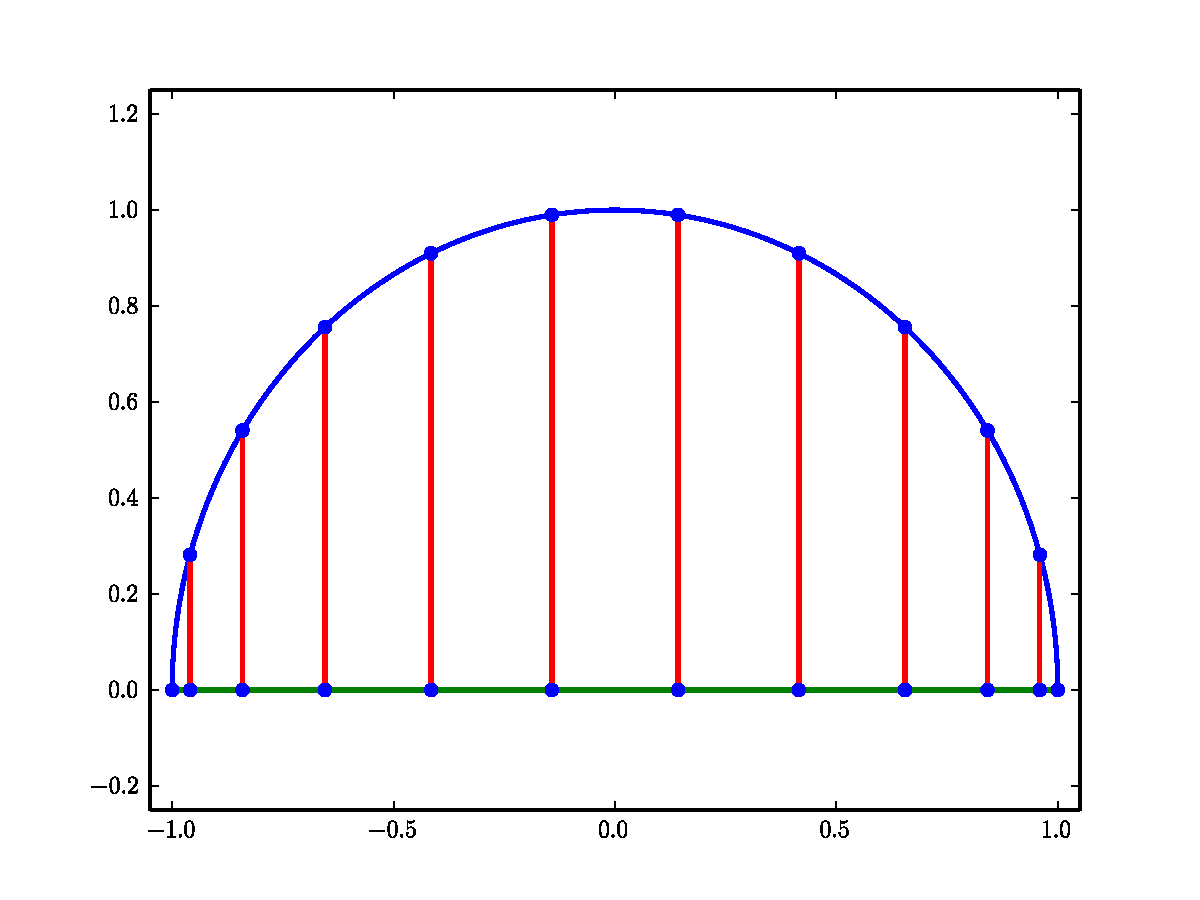
\includegraphics[width=\textwidth]{node_project.pdf}
\caption{The Chebyshev nodes are the projection of equispaced points on the upper half-circle onto the horizontal axis.
In Complex Analysis these points are known as the roots of unity.}
\label{fig:cheb_nodes_projection}
\end{figure}

\begin{figure}
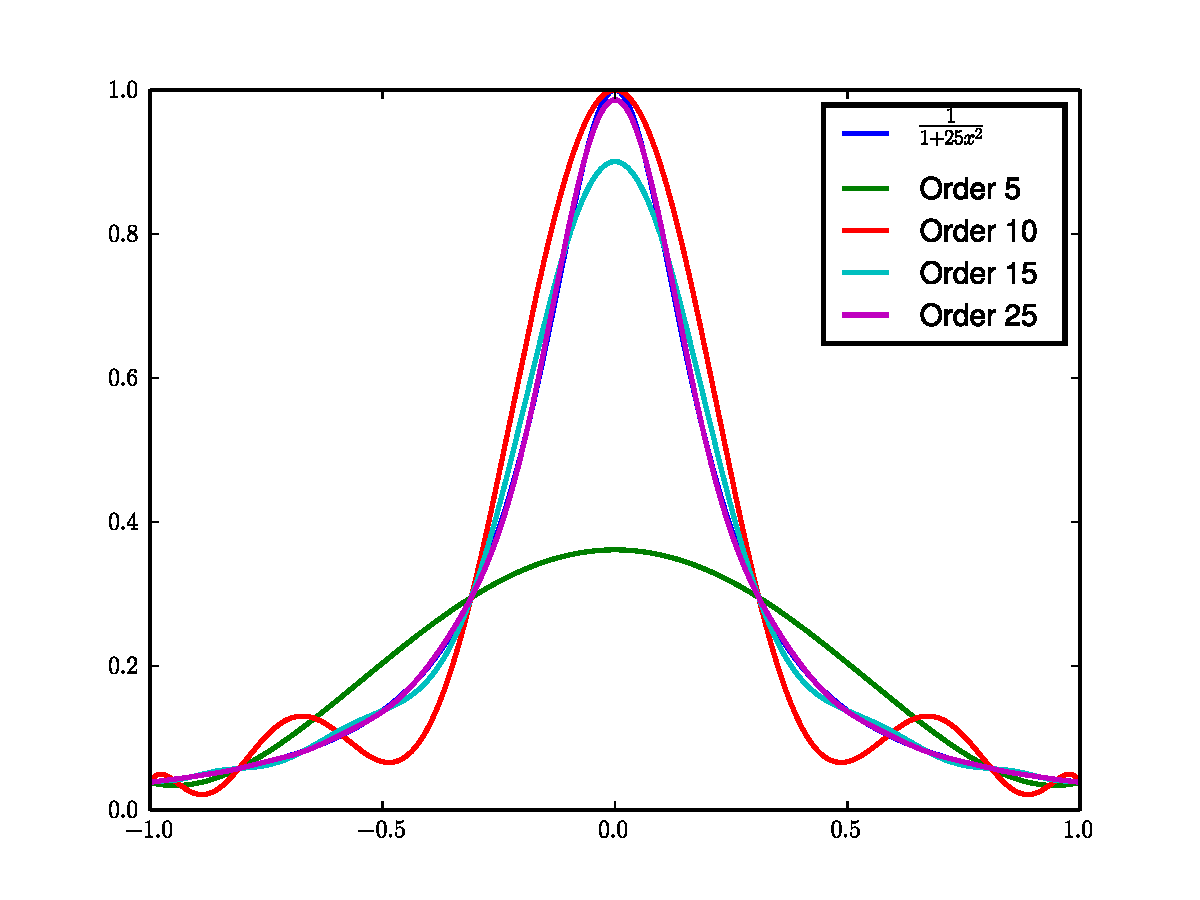
\includegraphics[width=\textwidth]{runge_chebyshev.pdf}
\caption{Different polynomial interpolants for the Runge function $\frac{1}{1 + 25 x^2}$ constructed by sampling at the Chebyshev nodes.}
\label{fig:runge_chebyshev}
\end{figure}

\begin{problem}
Write a function that, given the endpoints $a$ and $b$ of an interval and the order of the desired interpolating polynomial returns the $k+1$ Chebyshev nodes on the interval $[ a, b ]$.
Return them ordered from smallest to largest.
\end{problem}

\section*{Chebyshev Polynomials}
This sort of interpolation is also related to what are called the Chebyshev polynomials.
Chebyshev Polynomials can be used very nicely to approximate functions on $[ -1, 1 ]$ and, with proper scaling, can be used to approximate reasonably well-behaved functions on any interval.
The $k$'th Chebyshev polynomial is commonly written $T_k \left( x \right)$.
One way to define the Chebyshev Polynomials is that the $k$'th Chebyshev polynomial on the unit circle is the real part of the function $z^k$ on the unit circle.
More precisely, let $z(x) = t + i \sqrt{1 - x^2}$, then the $k$'th Chebyshev polynomial on $[-1, 1]$ is the real part of the polynomial $x^k$.
We can write this real part explicitly as
\[T_k \left( x \right) = \frac{1}{2} \left( z^k + z^{-k} \right) = \cos \left( k \cos^{-1} \left( x \right) \right)\]
Notice that, as this function has been defined, the Chebyshev polynomial of order $k$ on an interval takes values of $1$ and $-1$ at the $k+1$ chebyshev points corresponding to interpolation with a polynomial of order $k$ on that interval.
The first few Chebyshev polynomials are shown in Figure \ref{fig:cheb_polys}.

\begin{figure}
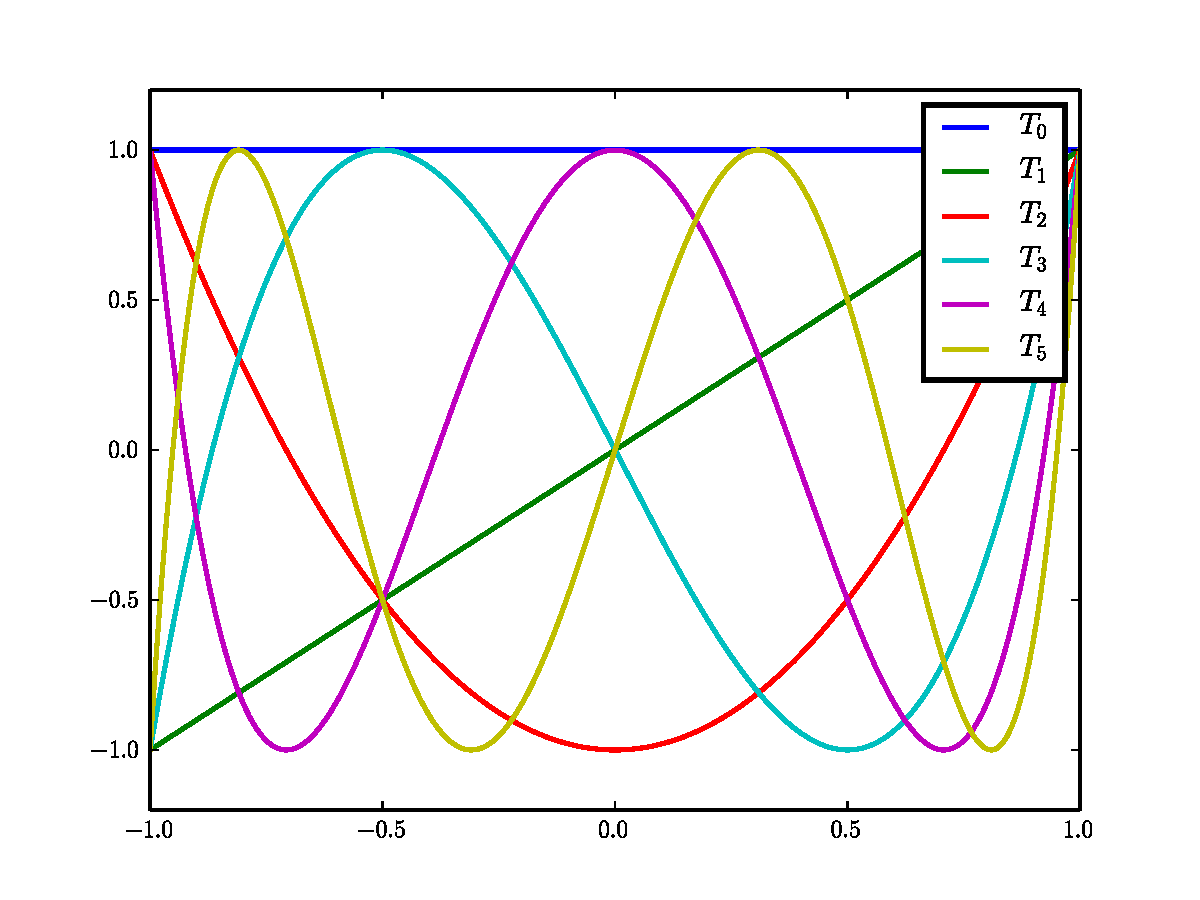
\includegraphics[width=\textwidth]{cheb_polys.pdf}
\caption{The first few Chebyshev Polynomials.}
\label{fig:cheb_polys}
\end{figure}

These polynomials are orthogonal with respect to the integral inner product
\[\langle f, g \rangle = \int_{-1}^1 \frac{1}{\sqrt{1 - x^2}} f\left( x \right) g\left( x \right) dx\]
This inner product allows us to write many functions as an infinite series of Chebyshev polynomials.
In particular, we can write any polynomial as a finite series of Chebyshev polynomials.
As it turns out, it is relatively easy to compute the Chebyshev series representation of an interpolating polynomial for a function on a given interval.
These approximations converge to the function we are approximating nearly as well as the partial sums of the infinite series formed using the inner product above, so, in practice, we will use them instead.

It can be shown that the Chebyshev polynomials follow the following recurrence relation: $ T_{k+1} \left( x \right) = 2 x T_k \left( x \right) - T_{k-1}$.
$T_0 \left( x \right)$ is equal $1$ and $T_1 \left( x \right)$ is equal to $x$ (still working on the interval $[-1, 1]$.)
This recurrence relation forms the basis for what is known as Clenshaw's Algorithm.
Clensaw's Algorithm says that, given a polynomial of degree $n$ represented as a sum of Chebyshev polynomials:
\[p\left(x\right) = \sum_{k=0}^{n} a_k T_k\left(x\right)\]
$p(x)$ can be evaluated by the recursion process outlined in Algorithm \ref{alg:clenshaw_recursion}.

\begin{algorithm}
\begin{algorithmic}[1]
\Procedure{ClenshawRecursion}{$X, c$}
	\State $u_{n+1} \gets 0$
	\State $u_{n} \gets a_{n}$
	\State $k \gets n-1$
	\While{$k \geq -1$}
		\State $u_k \gets 2 x u_{k+1} - u_{k+2} + a_k$
		\State $k \gets k-1$
	\EndWhile
	\State \pseudoli{return} $\frac{1}{2} \left( a_0 + u_0 - u_2 \right)$
\EndProcedure
\end{algorithmic}
\caption{Clenshaw Recursion}
\label{alg:clenshaw_recursion}
\end{algorithm}

The following recursion is equivalent to Algorithm \ref{alg:clenshaw_recursion}.
Let $u_{n+1} = 0$ and $u_{n} = a_n$ and $u_k = 2 x u_{k+1} - u_{k+2} + a_k$ for $k = n-1, n-2, \dots, 0$, then $p(x) = \frac{1}{2} \left( a_0 + u_0 - u_2 \right)$.

\begin{problem}
Write a Python function that performs Clenshaw's algorithm to evaluate a series of Chebyshev polynomials for an array of points in the interval $[-1, 1]$.
Use it to plot the first $5$ Chebyshev polynomials on that interval.
\end{problem}

\section*{Chebyshev Polynomials and Fourier Series}
In looking at the plots of the Chebyshev polynomials you may have noticed that the Chebyshev polynomials take alternating values of $1$ and $-1$ at the Chebyshev points on the interval $[-1,1]$ similar to how the functions $\cos\left(k x \right)$ change between $-1$ and $1$ on equispaced points in the interval $[ 0 , \pi ]$.
Recall that, as mentioned above, $T_k \left( x \right) = \cos \left( k \cos^{-1} \left( x \right) \right)$.
For discrete samples, this means that the Chebyshev coefficients for the interpolating polynomial through a function at the Chebyshev nodes has the same coefficients as the discrete cosine series would at the points $\cos^{-1} x$ where $x$ is a chebyshev node.
In practice this means we can compute an array of samples of a function at the Chebyshev nodes of the interval $[-1, 1]$, then compute the discrete cosine transform to get the corresponding coefficients to the Chebyshev interpolation.
This is very helpful since the discrete cosine transform is a close relative of the discrete Fourier transform.
\li{scipy.fftpack} and \li{pyfftw} both include discrete cosine transforms as \li{scipy.fftpack.dct} and \li{pyfftw.interfaces.scipy_fftpack.dct} respectively.
The discrete cosine transform is defined a little differently than the coefficients we need here.
There are several different versions of the discrete cosine transform.
Using the inverse discrete cosine transform of type 1 on an array $y$ of length $N$ will give us an array $x$ of values such that
\[y_k = z_0 + 2 \sum_{n=1}^{N-2} z_n \cos\left(\frac{\pi k n}{N-1}\right) + \left(-1\right)^k z_{N-1}\]
where $z = \frac{x}{2 \left(N - 1\right)}$.
To obtain the Chebyshev coefficients, we desire to find the vector $a$ of coefficients $a_n$ such that
\[y_k = \sum_{n=0}^{N-1} a_n \cos\left(\frac{\pi k n}{N-1}\right)\]
This means that, given the vector $x$, we can obtain $a$ by dividing all the terms of $x$ by $N-1$, and then dividing the first and last entries of $x$ by 2.
This means that we can obtain the coefficients of the Chebyshev interpolant using the following steps:

\begin{itemize}

\item Sample the function you desire to approximate at the Chebyshev nodes.
Make sure you use the sampled values in the order that corresponds to the chebyshev nodes when sorted in \emph{descending} order and not ascending order.

\item Compute the inverse discrete cosine transform of the data.
Use the option \li{type=1} to tell either scipy or pyfftw the version of the discrete cosine transform you want to use.

\item Divide all the coefficients by $\left( N - 1 \right)$ where $N$ is the number of nodes used.

\item Divide the first and last coefficient by $2$.

\end{itemize}

\begin{warn}
Often it is customary in computation to use values in ascending order.
When you compute the Chebyshev coefficients for the interpolatng polynomial through a set of points you will need the samples from the points sorted in descending order, not ascending order.
\end{warn}

\begin{problem}
Write a function that, given the samples for a function at the chebyshev nodes for a funciton on an interval computes the coefficients for the Chebyshev representation of the interpolating polynomial through the samples at the Chebyshev nodes.
\end{problem}

\section*{NumPy's Chebyshev Module}

NumPy includes a module for working with Chebyshev polynomials and Chebyshev series alongside its polynomials module.
It does not include all of the functions we had you write today, but it does include many other useful things.
This module includes a Python class for Chebyshev polynomials.
It works much like the poly1d class that is used for polynomials.
Here are a few lines of code that use NumPy's Chebyshev class to evaluate the 20'th Chebyshev polynomial.
We will plot the corresponding function using Matplotlib.
\begin{lstlisting}
import numpy as np
from numpy.random import rand
import numpy.polynomial.chebyshev as ch
from matplotlib import pyplot as plt
coefficients = np.zeros(20)
coefficients[-1] = 1
poly = ch.Chebyshev(coefficients)
X = np.linspace(-1, 1, 2001)
Y = poly(X)
plt.plot(X, Y)
plt.show()
\end{lstlisting}

Here we used the Chebyshev class to evaluate a Chebyshev series.
It also includes other methods that allow you to multiply, divide, differentiate, and integrate Chebyshev series.
We will discuss integration and differentiation later on.
There are also functions that allow you to convert back and forth between Chebyshev series and standard polynomials.

\begin{problem}
\label{prob:cheb_interpolations}
We will briefly consider the rate of convergence of these polynomial approximations.
Compute the coefficients for the interpolating Chebyshev series for the function $\cos x$ on the interval $[-1, 1]$.
This approximation converges very rapidly, so the first $20$ terms or so should be more than enough.
How many of these coefficients have absolute value greater than $10^{-14}$?
How close does your series approximate the actual function?

Now compute the coefficients for a degree $100000$ polynomial approximating the function
\[\sin \left( \frac{1}{x} \right) \sin \left( \frac{1}{\sin \left( \frac{1}{x} \right)} \right) \]
on the interval $[-1, 1]$.
How large are the last $10$ coefficients in the series?
Use NumPy's Chebyshev class to plot this function at $100001$ equispaced points on the interval $[-1, 1]$.
Plot it with the original function.
Compare the two.
How close are they?
Notice how the interpolating polynomial is able to approximate the original function about as well as the discrete sample of the original function.
\end{problem}

Problem \ref{prob:cheb_interpolations} also illustrates an interesting principle.
These series converge more quickly when a function is infinitely differentiable everywhere in the complex plane (the proper term for a function like this is "entire").
For functions that do not satisfy this property, it can be shown (roughly speaking) that the rate of convergence depends on how many times differentiable the function is on the interval of interpolation.
For a less well-behaved function like the one considered in the second half of Problem \ref{prob:cheb_interpolations} the coefficients converge much more slowly.
The last $10$ coefficients for the interpolant of degree $2^{23} - 1$ are still
\begin{lstlisting}
[9.52973125e-08,  -1.89451973e-09,  -7.42182166e-08,
 1.89319137e-09,   5.26564839e-08,  -1.89451836e-09,
 -3.13050802e-08,   1.89319005e-09,   1.03700608e-08,
 -9.47258778e-10]
\end{lstlisting}

% We could add in a problem where they interpolate the PDF of the standard normal distribution and use it to estimate the CDF at different values.
% Given a proper setup, such an approximation gives correct answers to machine precision in about the same amount of time as the version in Scipy.stats.
% The only limitation is that the interpolant is limited to a specific interval instead of allowing approximation anywhere.
% That isn't much of an issue though since the PDF is practically 0 outside a reasonably-sized interval anyway.
